\ifgerman{\chapter{Vorgeschlagene Methoden}}{\chapter{Modeling performance estimation as a learning process}}
\label{methods}

The currently existing performance estimators recalled in the previous chapter are made up of two groups. The first kind only uses information available for the already trained classifier; the cross-validation and bootstrapping family belong to it. The other one collects information during the classifier's training, using it to fit and extrapolate a learning curve. How that information is obtained differs, common practices include the use of holdout test sets and k-fold cross-validation \cite{FigueroaEtal2012}.

The methods evaluated in this thesis build on both approaches. Generalizing the extrapolating approach, estimating the performance of a classifier based on individual estimates is a type of learning itself, falling into the category of \textit{regression} since performance is not discreet. But instead of using the classifier's journey, the combined estimator simulates different training sets that could have been an earlier state of the classifier, i.e. the subsets of the current training set. To help illustrating this method, the following scenario is assumed: a dataset composed of both labeled and unlabeled data $\mathcal{D} = \mathcal{L} \cup \mathcal{U}$ with $\mathcal{L} = \{(\vec{x}_i, y_i) : i \in \{1, ..., n\}\}$ and $\mathcal{U} = \{(\vec{x}_i, .) : i \in \{n+1, n+2, ...\}\}$, $y \in \{0, 1\}$, serves as the basis for an active learner, which selects a training set $X \subseteq \mathcal{L}$ of size $k \leq n$. This set is used to train a classifier $c_X: \vec{x} \mapsto y$. We now would like to know the accuracy $acc_c(X, \mathcal{D})$ the classifier has on the entire dataset.

\section{Performance estimation on training sub-sets}

\begin{table}[h]
\centering
\begin{tabular}{c | C{8cm}}
Symbol & Description\\
\hline
$\mathcal{D}$ & Whole dataset\\
$\mathcal{U}$ & Unlabeled part of $\mathcal{D}$\\
$\mathcal{L}$ & Labeled part of $\mathcal{D}$\\
$X$ & Current training set\\
$k$ & Size of $X$: $k = |X|$\\
$\vec{x}_i$ & Instance of $X$: $\vec{x}_i \in X \forall i=\{1,...,k\}$\\
$y_i$ & Class label of instance $\vec{x}_i$\\
$c_X$ & Classifier trained with set $X$\\
$acc_c(A,B)$ & True accuracy of classifier $c$ trained with set $A$ on the instances $B$\\
$\widehat{acc}_c(A,B)$ & Estimate of $acc_c(A,B)$\\
$S^j_i$ & $i$th subset of $X$ with size $j$\\
$\check{S}$ & Selected subsets of $X$ from capped sub-sampling\\
$\tilde{S}$ & Set of paths (n-tuples of size $k-1$)\\
$T, \check{T}, \tilde{T}$ & Test sets $X \setminus S^j_i$ for estimation\\
$Y_m$ & Set of tuples containing a subset estimate and the subset's size; input of the fitting algorithm\\
$f^m(j)$ & Function fitted using $Y_m$ depending on $j$ as the classifier's training set size\\
$H_i$ & Holdout test sets\\
$\mathcal{X^k}$ & Set containing all training sets of size $k$ used for testing\\
$K$ & Kernel for KDE\\
$h$ & Bandwidth for KDE\\
\end{tabular}
\caption{List of symbols and their meaning}
\label{tab:tos}
\end{table}

In order to obtain the performance estimates for the classifier trained on training subsets, \textit{leave-p-out (LPO) cross-validation} with $p \in \{1,...,k-1\}$ is used. As $p$ is the number of omitted and thus test instances, the training subsets $S^{k-p}_i \subset X$ are of size $|S^j_i| = j$ and $i = \{1,...,{k \choose j}\}$, resulting in ${k \choose p}$ accuracy estimates for each subset size. The corresponding test sets are $T^{k-p}_i = X \setminus S^{k-p}_i$. While LPO is a pessimistic estimator when applied to a classifier with training set size $k$, i.e. it systematically places the accuracy lower than its true value, it is \textit{unbiased} for a classifier with a training set of size $k-p$ \cite{RodriguezEtAl2013}. This leaves us with $2^k-2$ estimates in total, each of them unbiased, but at the cost of exponential time complexity; some sort of selection may be reasonable to reduce it.

Another option with regard to the estimation is \textit{bootstrapping}. It offers a little more variety, as different types like \textit{na\"{i}ve}, \textit{leave-one-out} and \textit{.632} are available. Also, individual estimates are more expensive to compute, as multiple bootstrap samples are first created. Also, there is no real equivalent to LPO for bootstrapping, meaning that the estimation looks slightly different: for \textit{leave-one-out (LOO) bootstrapping}, an estimate for a subset $S^j_i$ and a corresponding bootstrap sample is actually the average of $j$ estimates, holding out each of the $j$ instances once and testing the resulting classifier on the hold-out instance. That is how bootstrapping was defined originally, anyway; however, the instances in $T^j_i$ not used for training would be left out. As they are not part of the training, they may as well be used as a test set. Problematic is that .632 bootstrap relies on a ratio of expected pessimism and expected optimism of LOO's estimate and the classifier's training error respectively. This is based on the probability of one instance not occurring in $n$ draws with replacement, i.e. how likely it is that a bootstrap sample does not contain a given instance. Since the instances in $X \ S^j_i$ cannot possibly occur in the bootstrap sample, which is drawn from $S^j_i$, the bootstrap estimate should be less pessimistic and the ratio may not hold anymore.

\subsection{Sub-sampling of fitting points}
Regardless of which estimation technique is used, the complexity still scales exponentially with the training set size $k$. To reduce the amount of estimates for the model fitting process, some sort of selection has to occur. In this section, three sub-sampling strategies are explored. However, it is to be kept in mind that reducing the information available naturally has some drawbacks, including an expected higher variance and, if not done properly, an added bias. Also, the sampling may influence the fitting itself, potentially inflicting additional penalties to the robustness.

A simple, yet effective method which will be called \textit{capped sub-sampling} is to cap the number of estimates. Possible options are to either impose a fixed, hard cap for all training set sizes $k$, or to use a polynomial dependent on it, e.g. $k^2$. A potential pitfall is the selection of the remaining subsets: selecting either randomly over all possible subsets or from pools for each subset size $k-p$ with sizes proportional to $k \choose p$ prevents unintentional importance assignment to subset sizes. The computation of this reduced set $\check{S} \subseteq S$ is illustrated in \ref{alg:cappedSubSampling}, the corresponding test sets $\check{T}^j_i = X \setminus \check{S}^j_i$.

\begin{algorithm}[h]
	\begin{algorithmic}[1]
		\State {$X = \left\{(\vec{x}_, y_1),...,(\vec{x}_k, y_k)\right\}$}
		\Comment {Current training set}
		\State {$numOfSamples \gets ...$}
		\State {}
		\State {$S \gets powerset(X)$}
		\Comment {Compute all possible subsets}
		\State {}
		\State {$\check{S} \gets \emptyset$}
		\For {$j \gets 1$ $to$ $k-1$}
		\For {$i \gets 1$ $to$ $numOfSamples$}
		\State {$currSample \gets drawWithoutReplacement(S^j)$}
		\Comment {Get a random subset of size j and remove it}
		\State {$\check{S} \gets \check{S} \cup currSample$}
		\EndFor
		\EndFor
	\end{algorithmic}
	\caption{Pseudocode for capped sub-sampling}
	\label{alg:cappedSubSampling}
\end{algorithm}

A related approach exports the computational cost to the fitting process. Instead of selecting multiple subsets $S^j_i$ per size once and using them as a basis for one model, this sub-sampling creates multiple models and selects only one subset $S_j$ per $j$. Formally, we have a tuple $\tilde{S_i} = (s^1,...,s^{k-1})$ with $i \in \{1,...,r\}$ and $s^j \in S^j$, which will be called a \textit{path}. Their respective test sets are $\tilde{T}_i = (X \setminus s^1,...,X \setminus s^{k-1})$. The $S_j$ can be drawn with or without replacement, although the latter may lead to a lower variance, as seeing the same constellation multiple times does not add information, whereas a different one does. The parameter $r$ is up to choosing, with an upper limit of $\prod_{i=1}^{k-1} {k \choose i}$ as the number of combinations for drawing with replacement; the algorithm for this is depicted in \ref{alg:unresPathSubSampling} and goes by the name of \textit{path sub-sampling}. This would result in a higher complexity than exponential, namely $O(k!)$. However, accounting for all possible subset combinations may not be necessary, as there are far less unique combinations of accuracy estimations. This is due to the number of test instances available for a given training subset. For example, a classifier trained on a set of size one tested against a set of size three will have four potential test outcomes: either one, two, three or none instances were correctly classified, resulting in an estimated accuracy of $\frac{1}{3}, \frac{2}{3}, 1$ and $0$, respectively. As a growth in size of the training set in turn causes a reduction in size of the test set, the amount of potential accuracies $\widehat{acc}_c(S^j_i, T^j_i)$ shrinks from $k$ to $2$ for $j = \{1, ..., k-1\}$. Thus, the number of unique combinations would shrink to $k!$.

\begin{figure}[h]
	\centering
	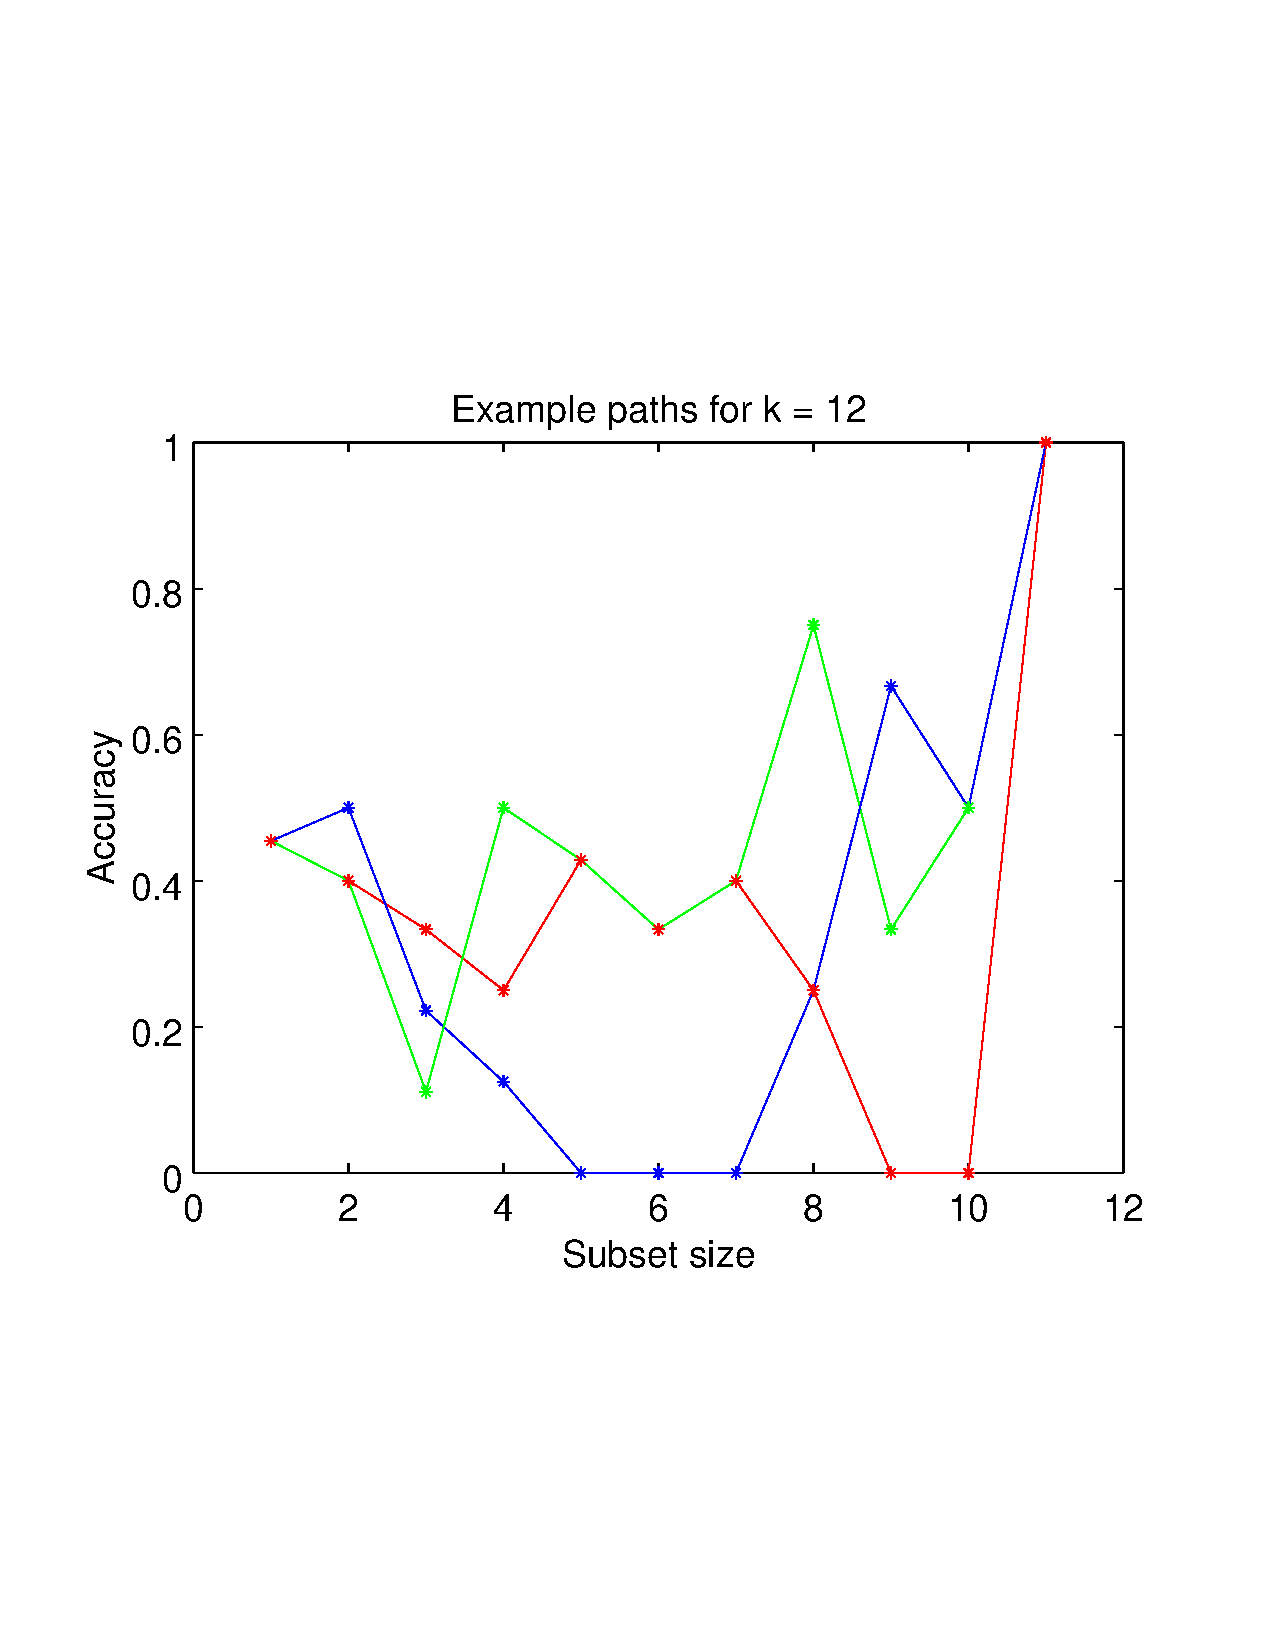
\includegraphics[trim = 0cm 6cm 0cm 5cm, clip = true, width = 0.45\textwidth]{pathExample1}
	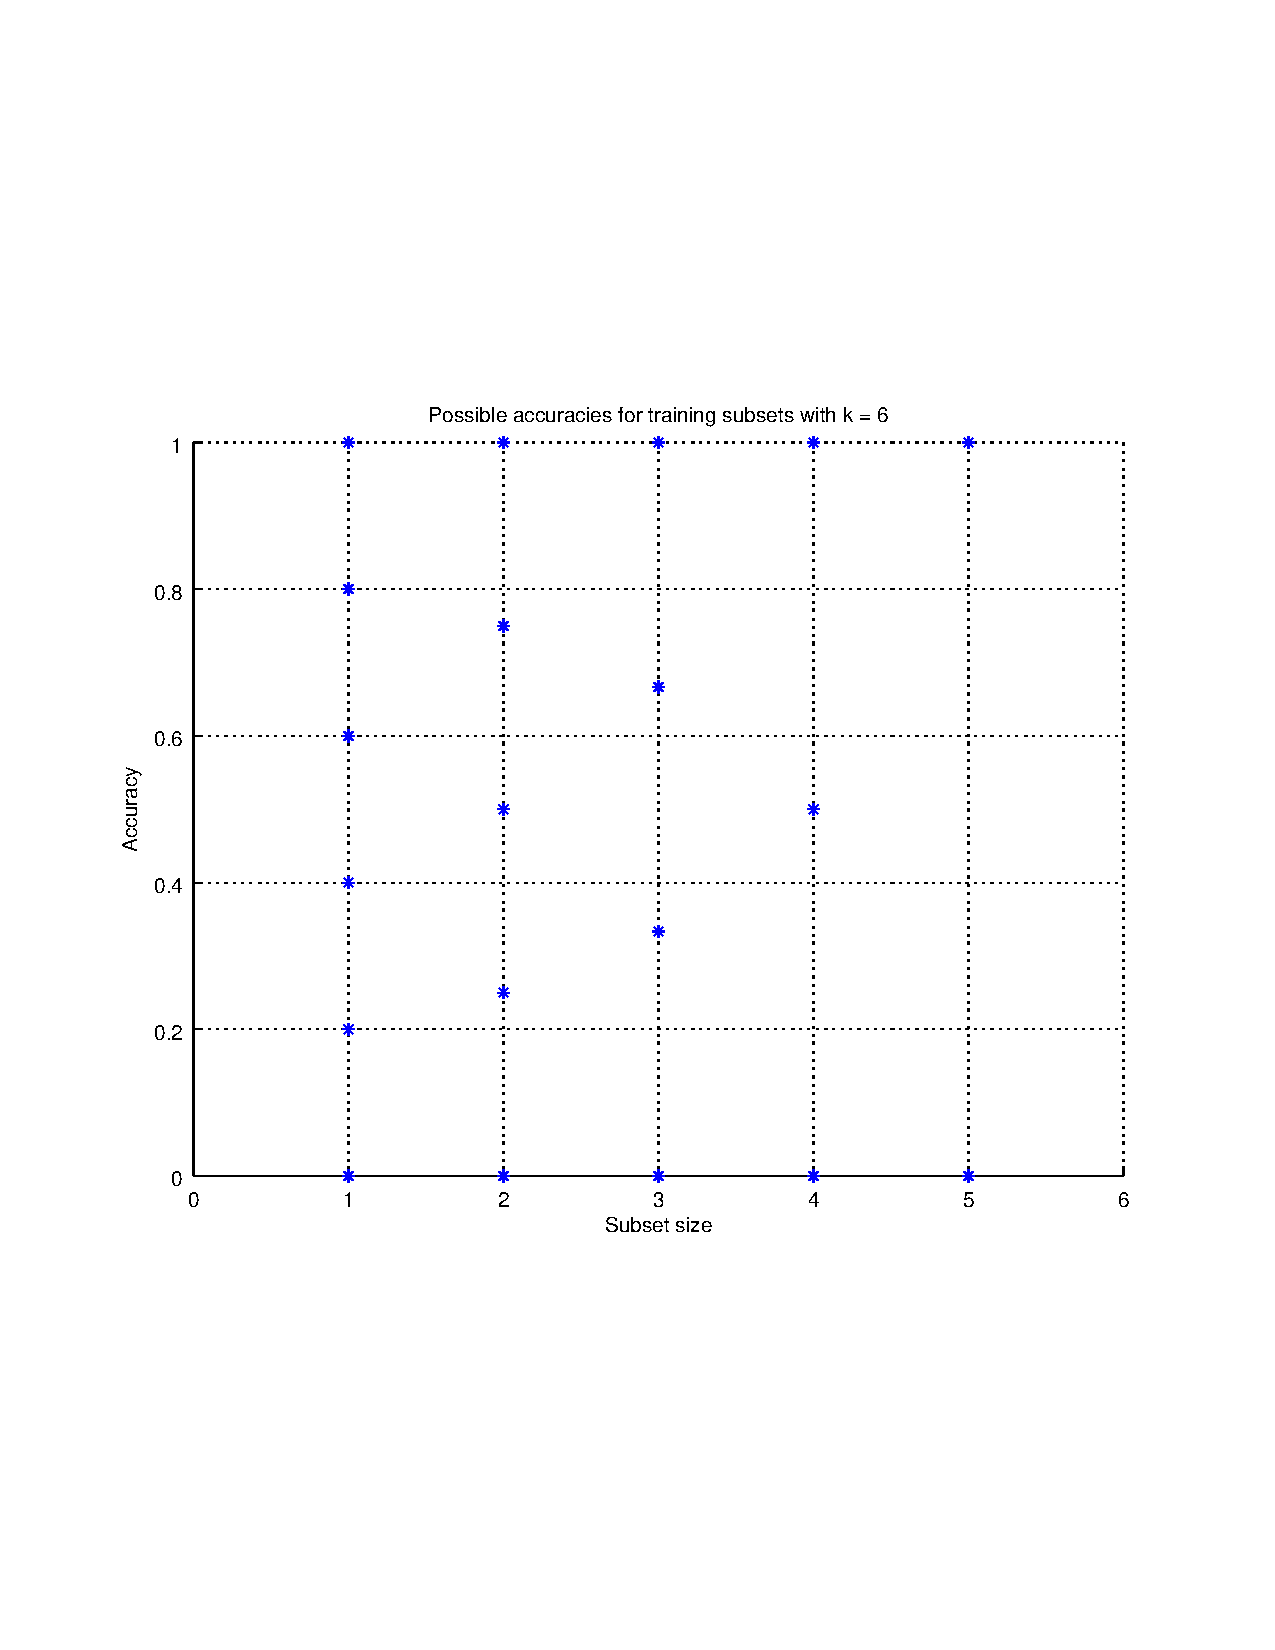
\includegraphics[trim = 0cm 6cm 0cm 5cm, clip = true, width = 0.45\textwidth]{accDemonstration}
	\caption{Left: Three example paths generated with path-superset sub-sampling. The zigzag shape illustrates the difficulties for the fitting. Right: All possible accuracies for training subsets with $k = 6$}
	\label{fig:pathAccExamples}
\end{figure}

Since the actual realization of the accuracies is not yet known, they would have to be computed first. This means that this approach is inept to reduce the number of needed subsets, but the idea of using multiple models instead of only one is still valid; it may increase the spread of the final estimate $\widehat{acc}_c(X, \mathcal{D})$ due to the reduced information available for each model, but also allows to derive a distribution for the accuracy (see \ref{evaluation:objective}).

Following this, there are other possible restrictions with regard to the selection of the paths $\tilde{S_i}$. As it is, randomly taking subsets of each size allows for instances present in $S^j$ to not be selected for the larger sets $S_{j+1},S_{j+2},...$. However, a classifier trained by an active learner does not usually discard previously selected instances. Thus, it seems logical to restrict subsets of larger size to be supersets of their predecessors $S^j \subset S^{j+1}$; see \ref{alg:resPathSubSampling} for the pseudocode. This again reduces the possible combinations to $k!$, as the sampling from $X$ is now done without replacement. This time, however, the estimates for every subset are not needed because each path is equally likely, meaning that this sub-sampling is applicable even without precomputing the estimates. This assumption only holds in general for random sampling; other active learners may show preferences for some instances which, in their eyes, improves the classifier's performance the most. Due to its restriction of the possible paths this method will be referenced as \textit{path-superset sub-sampling}.

\begin{algorithm}[h]
	\begin{algorithmic}[1]
		\State {$X = \left\{(\vec{x}_, y_1),...,(\vec{x}_k, y_k)\right\}$}
		\Comment {Current training set}
		\State {$numOfPaths \gets ...$}
		\State {}
		\State {$S \gets powerset(X)$}
		\State {}
		\State {$\tilde{S} \gets \emptyset$}
		\For {$i \gets 1$ $to$ $NUM\_OF\_PATHS$}
		\State {$currPath \gets nTuple(k)$}
		\For {$j \gets 1$ $to$ $k-1$}
		\State {$currPath_j \gets drawRandom(S^j)$}
		\Comment {Get a random subset of size j}
		\EndFor
		\State {$currPath_k \gets i$}
		\Comment {The same path may get drawn multiple times,}
		\State {}
		\Comment {but it still has to be in the set}
		\State {$\tilde{S} \gets \tilde{S} \cup currPath$}
		\EndFor
	\end{algorithmic}
	\caption{Pseudocode for path sub-sampling}
	\label{alg:unresPathSubSampling}
\end{algorithm}

\begin{algorithm}[h]
	\begin{algorithmic}[1]
		\State {$X = \left\{(\vec{x}_, y_1),...,(\vec{x}_k, y_k)\right\}$}
		\Comment {Current training set}
		\State {$numOfPaths \gets ...$}
		\State {}
		\State {$S \gets powerset(X)$}
		\State {}
		\State {$\tilde{S} \gets \emptyset$}
		\For {$i \gets 1$ $to$ $NUM\_OF\_PATHS$}
		\State {$currPath \gets nTuple(k)$}
		\For {$j \gets 1$ $to$ $k-1$}
		\State {$validSubsets \gets contains(S^j, currPath)$}
		\Comment {Limit the available subsets to supersets of the current path}
		\State {$currPath_j \gets drawRandom(validSubsets)$}
		\Comment {Get a random subset}
		\EndFor
		\State {$currPath_k \gets i$}
		\Comment {The same path may get drawn multiple times,}
		\State {}
		\Comment {but it still has to be in the set}
		\State {$\tilde{S} \gets \tilde{S} \cup currPath$}
		\EndFor
	\end{algorithmic}
	\caption{Pseudocode for path-superset sub-sampling}
	\label{alg:resPathSubSampling}
\end{algorithm}

\subsection{Extracting learning curves from performance estimates}
Now that the subsets have been selected, the individual performances have to be estimated. This requires a classifier being trained on each of them and testing it on the corresponding test set. After that comes the decision of which estimates to use to fit one or more learning curve models, and how. The algorithm doing the fitting takes a set of tuples $Y_m = {(a,j)}$ with $j \in \{1,...,k-1\}$ and $a \in [0,1]$. As a result it outputs a function $f^m: \mathbb{N} \mapsto \mathbb{R}$. There are multiple options available for how the $Y_m$ are chosen:
\begin{itemize}
	\item \textbf{Mix grouping}: In the most simple case, there is only one $Y = \{(\widehat{acc}_c(\check{S}^j_i, \check{T}^j_i), j): j\in\{1,...,k-1\}, i\in\{1,...,|\check{S}^j|\}\}$: every subset estimate is taken and given to the fitter, producing a single function $f^1$.
	\item \textbf{Averaged grouping}: As originally intended for leave-p-out estimation, the subset estimates are first averaged before passed to the fitting:\\$Y = \{(\frac{1}{|S^j|} \sum_{i=1}^{|S^j|} \widehat{acc}_c(S^j_i, T^j_i), j): j \in \{1,...,k-1\}\}$. This also results in only one function, but takes some strain away from the fitting. Problematic may be that the amount of estimates for any subset size $j$ does not vary anymore, withholding information from the fitting.
	\item \textbf{Path grouping}: For path or path-superset sub-sampling, $m$ equals the number of paths $|\tilde{S}$ selected. Each $Y_m$ then contains $k-1$ estimates: $Y_m = \{(\widehat{acc}_c(\tilde{S}_{m,i}, \tilde{T}_{m,i}), m): i \in \{1,...,k-1\}\}$. This results in multiple functions $f^m$.
\end{itemize}

\section{Combining sub-estimates with curve fitting}

\subsection{Function models and fitting algorithms}
\label{methods:function_models}
The function model used has to be capable of modeling the learning process and also largely determines the spectrum of algorithms available. For a linear model or one that can be linearized, e.g. the 2-parameter exponential law, the computation of the parameters which minimize the squared error is well known and trivial. More complex algorithms are necessary for functions which cannot be linearized, like the 3-parameter exponential law. Then, iterative methods have to be used, like the Levenberg-Marquardt algorithm \cite{Levenberg1944}. It works by iteratively adapting the parameters following its approximated gradient, with the goal to find a minimum for the least squares error function.

While they are able to handle a larger number of functions, they also need to be provided with various tuning parameters. In the case of Levenberg-Marquardt, initial values and maximal change per parameter as well as the partial derivatives w.r.t. the parameters must be given. Also, convergence is not guaranteed; unlike linear least squares, where minimizing parameters exist for at least two data points with different x components, poorly chosen initial parameters or too few iterations may lead to divergence. Potentially even more detrimental are local minima, as a divergence may be recognized. Here, the derivative of the error function is zero, indicating a minima, but different ones with lower absolute error values exist. However, the algorithm has no way of detecting this; the only options to avoid such a, quite literal, pitfall are to try the fitting with multiple initial parameters, hoping to get lucky, or to exploit previous knowledge about the data.

Potential function models were examined in section \ref{background}, especially in \cite{Singh2005}. A good candidate for least squares fitting seems to be the 3-parameter exponential law in \ref{eq:expFunc}.
\begin{equation}
\label{eq:expFunc}
f_{E}(x) = a + b \cdot e^{c \cdot x}
\end{equation}
Unfortunately, it falls in the category "non-linearizable" and requires iterative fitting. A similar function class are sigmoids. The evaluation in \ref{evaluation} investigates the characteristics of the sigmoid in \ref{eq:sigFunc} in comparison to \ref{eq:expFunc}.
\begin{equation}
\label{eq:sigFunc}
f(x)_{S} = y_0 + 2 \cdot (y_0 - S) \cdot \left( \frac{1}{1+e^{m \cdot x}} - 0.5 \right)
\end{equation}
While it was not part of the testing in the cited articles, it can be similar in shape thanks to the exponential part and has the advantage of semantic parameters, that means they communicate the function's shape without the need to draw it. In this case, $y_0$ indicates the y-intercept, $S$ is the asymptotic threshold, and $m$ communicates the function's slope. This way, it is easier to find appropriate bounds for the parameters during fitting: clearly, a learning curve has to have both y-intercept and asymptote between 0 and 1 as well as a slope larger or equal to 0. While similar parameters can be found for the exponential function, they are not as precise, leaving more room for potentially wrong guessing, especially for the initial parameters.

As overfitting is a real possibility for all kinds of learning \cite{Dietterich1995}, the third function tested is the simple linear model of form
\begin{equation}
\label{eq:linFunc}
f(x)_{L} = a + b \cdot x
\end{equation}
Since it does not approximate a whole learning curve of bent shape as seen in \ref{fig:curve_general}, it will only be fit on accuracy estimates for subsets of size $j \in \{k-5,...,k-1\}$, simply discarding the others. Thus, the linear fit approximates the momentary gradient of the classifier's accuracy rather than the whole process. \ref{fig:allFunctions} exemplifies the general shape of all three functions when fit on data.

\begin{figure}[h]
	\centering
	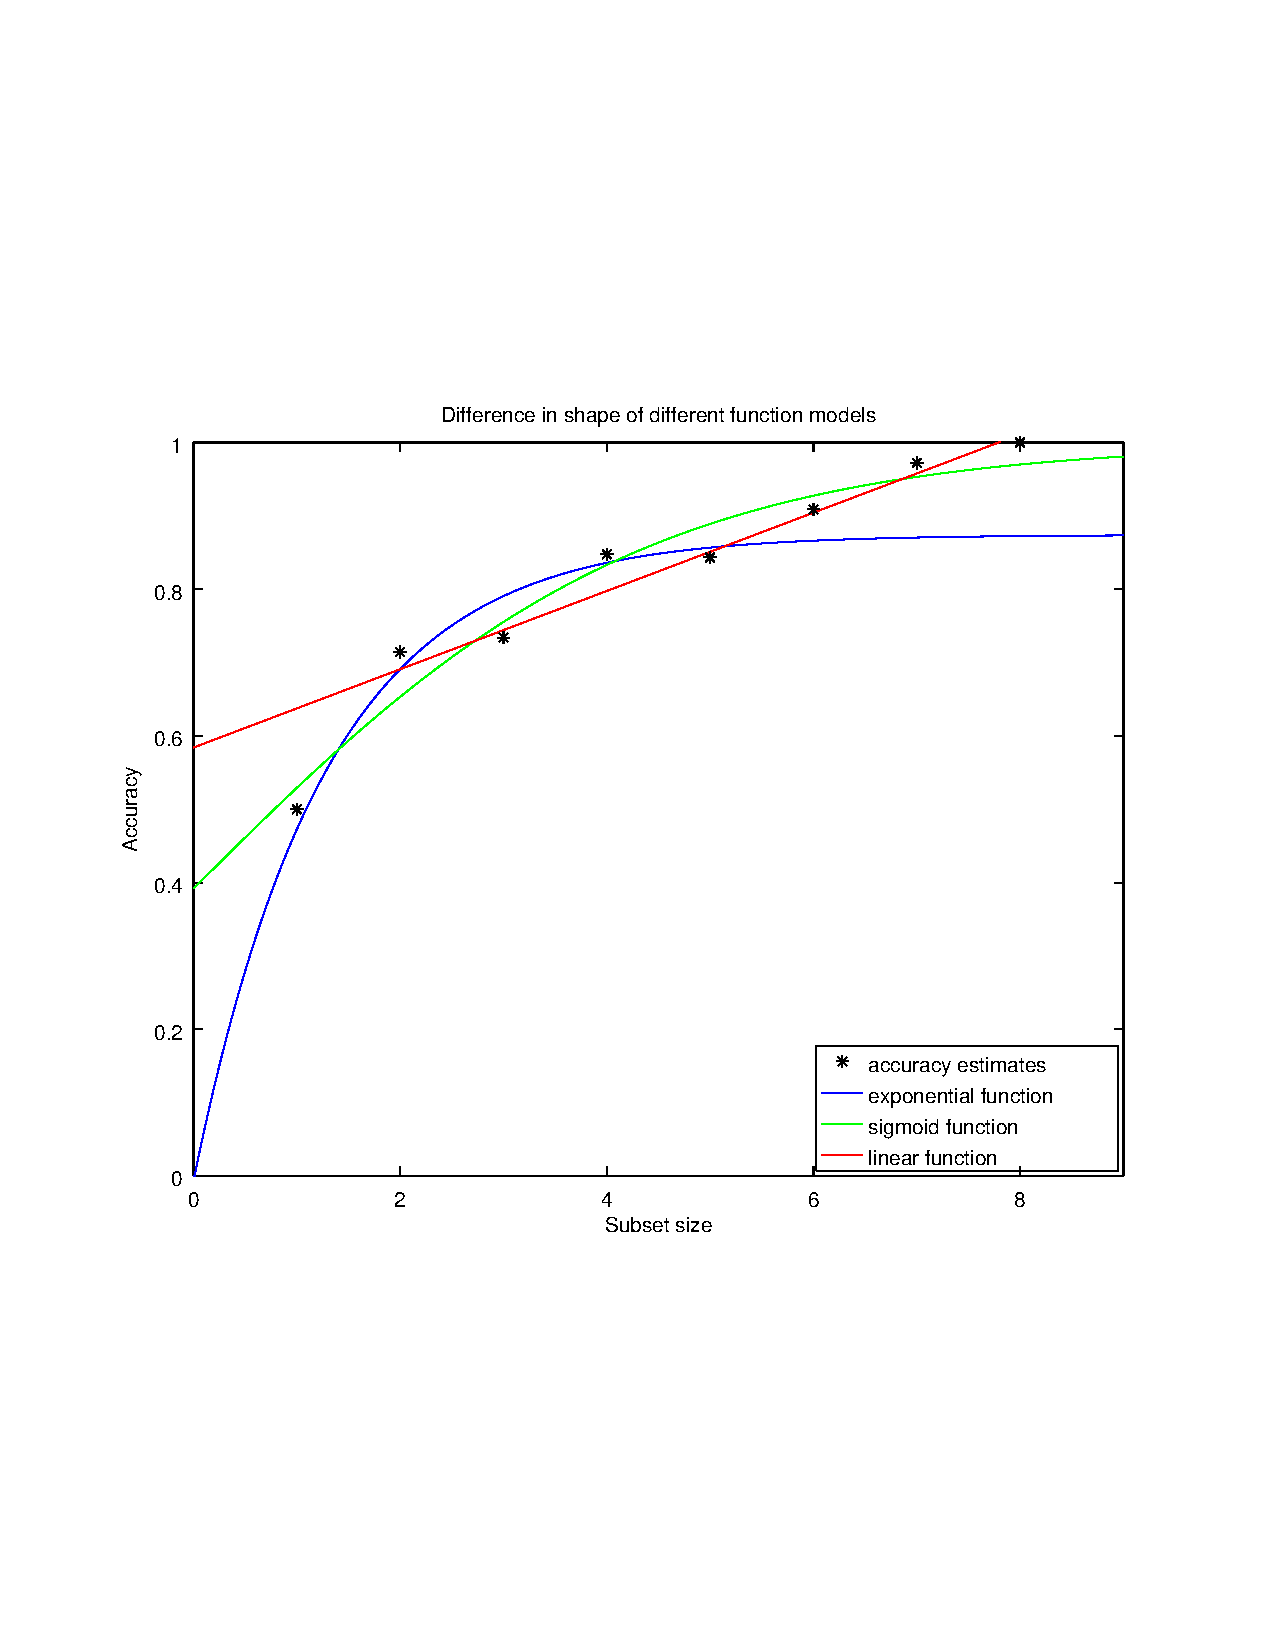
\includegraphics[trim = 0cm 6cm 0cm 5cm, clip = true, width = 0.7\textwidth]{allFunctions}
	\caption{The shape of the three function models fit on example estimates produced by \textit{averaged grouping} with $k = 9$ for the \textit{seeds} dataset}
	\label{fig:allFunctions}
\end{figure}

The final performance estimate for our classifier $c_X$ is then obtained by extrapolating the functions $f^m$, i.e. $\widehat{acc}_c(X, \mathcal{D}) = \frac{1}{|f|} \sum_{i=1}^{m} f^m(k)$. In case of $|f| > 1$ the $f^m(k)$ can be used as samples of a probability distribution, opening up the possibility of comparing not only the difference of $\widehat{acc}_c(X, \mathcal{D})$ to $acc_c(X, \mathcal{D})$, but also how different the (estimated) distributions of $acc_c$ over $\mathcal{(D)}$ are, which is explained in detail in \ref{evaluation:objective} as part of the measurements used to compare the different estimators.

\subsection{Tuning the model fitting}
Usually, data gathered for curve fitting is not uniform, e.g. some data points are more likely to be tainted with error or do not carry much information. An example could be a study questioning people about the value of the elementary electric charge. With a sufficiently large sample size, averaging the individual statements may produce a fairly rough approximation to the real value. However, if the answers of people related to physics (students, engineers etc.) would be counted twice, the approximation would likely be better, as these people generally know more about physics and are thus more likely to know the correct answer.

A similar situation presents itself when using averaged grouping, where the subset estimates $\widehat{acc}_c(S^j_i, T^j_i)$ for each $j$ are first averaged, then sent to the fitting algorithm. However, this procedure omits how many estimates were originally present, which is quite important information; more estimates mean the resulting average should be less noisy. This is where statistical weights come into play: they inform the fitting algorithm about how important a low error of the fitted function for a given data point is, the difference in shape for an example exponential function is depicted in \ref{fig:weigthingExample}: the weighted curve is flatter since the more extreme points at $x = 1$ and $6$ have less influence. Assigning weights proportional to the amount of estimates that went into each $Y_{m,i}$ may ensure that less noisy data influences the shape of the curve more heavily.

\begin{figure}[h]
	\centering
	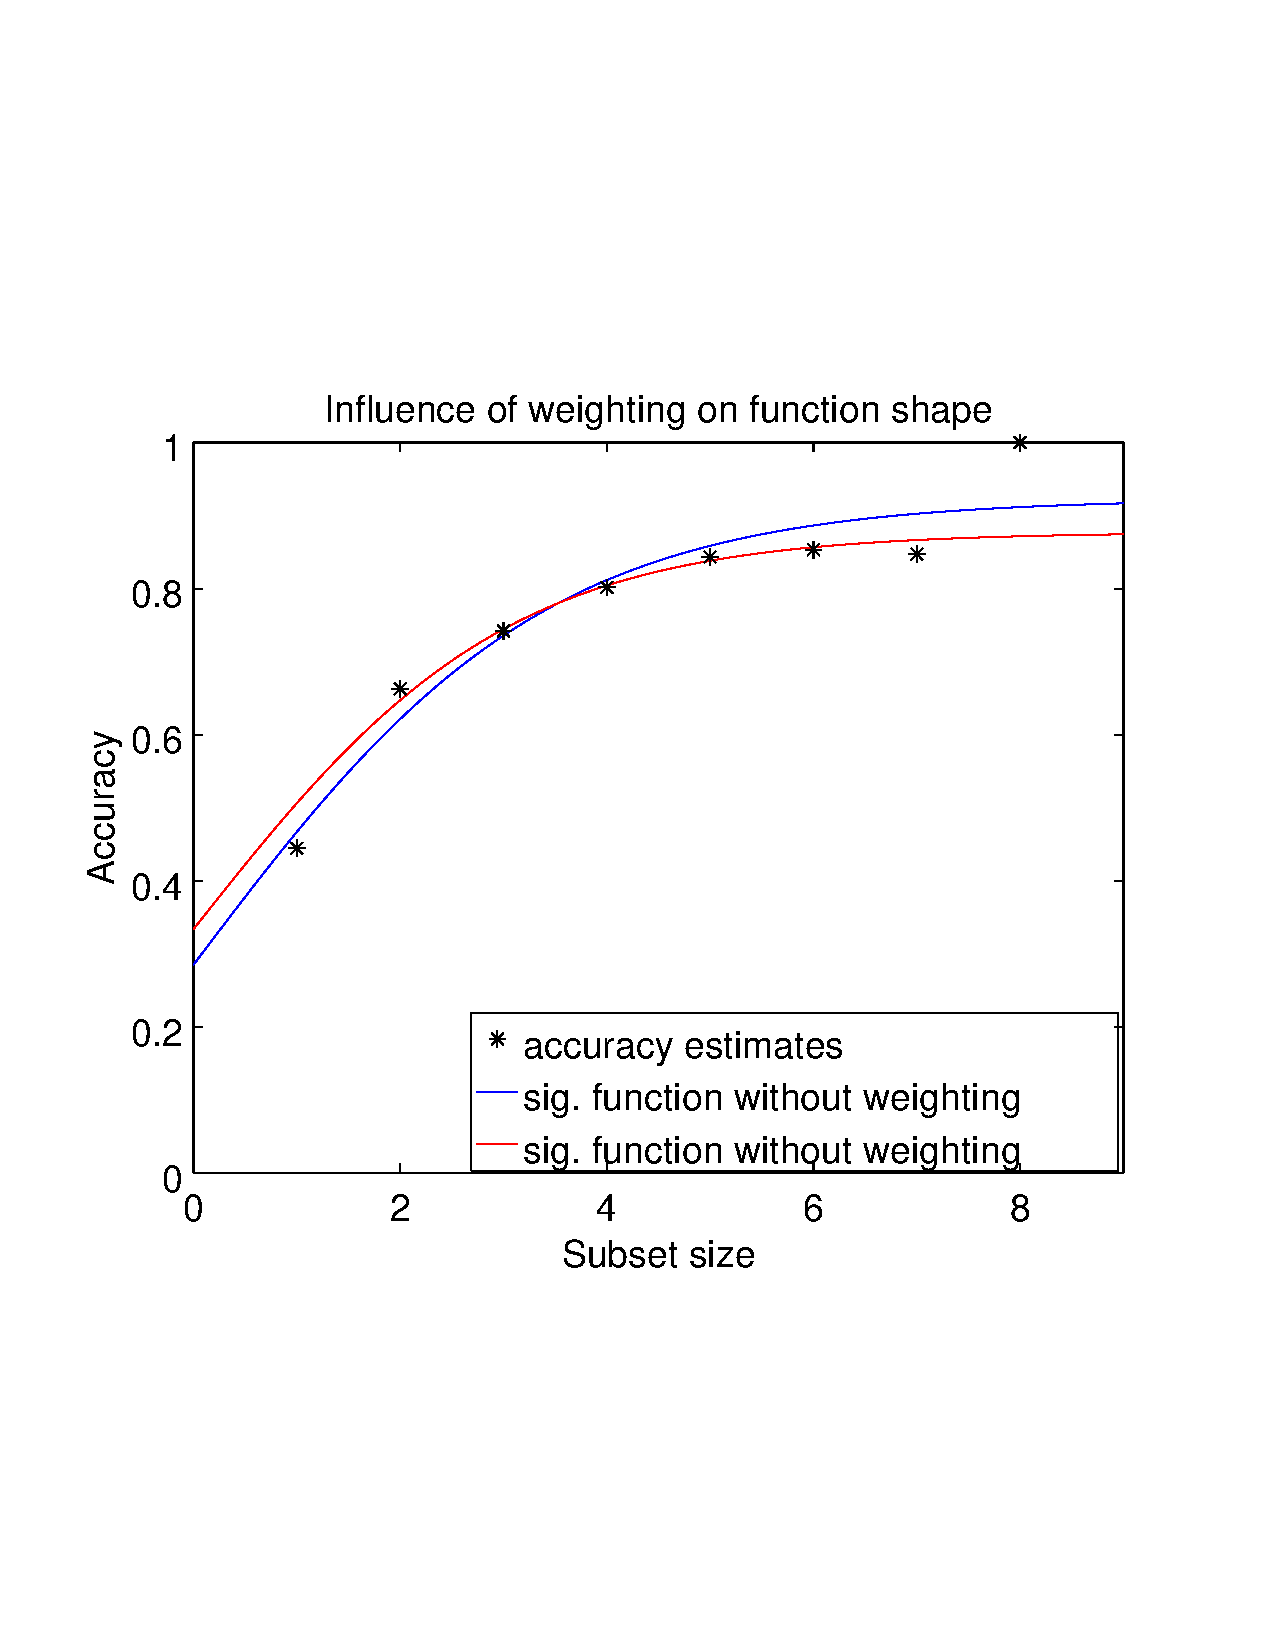
\includegraphics[trim = 1cm 7cm 1cm 6cm, clip = true, width = 0.48\textwidth]{weightingDiff}
	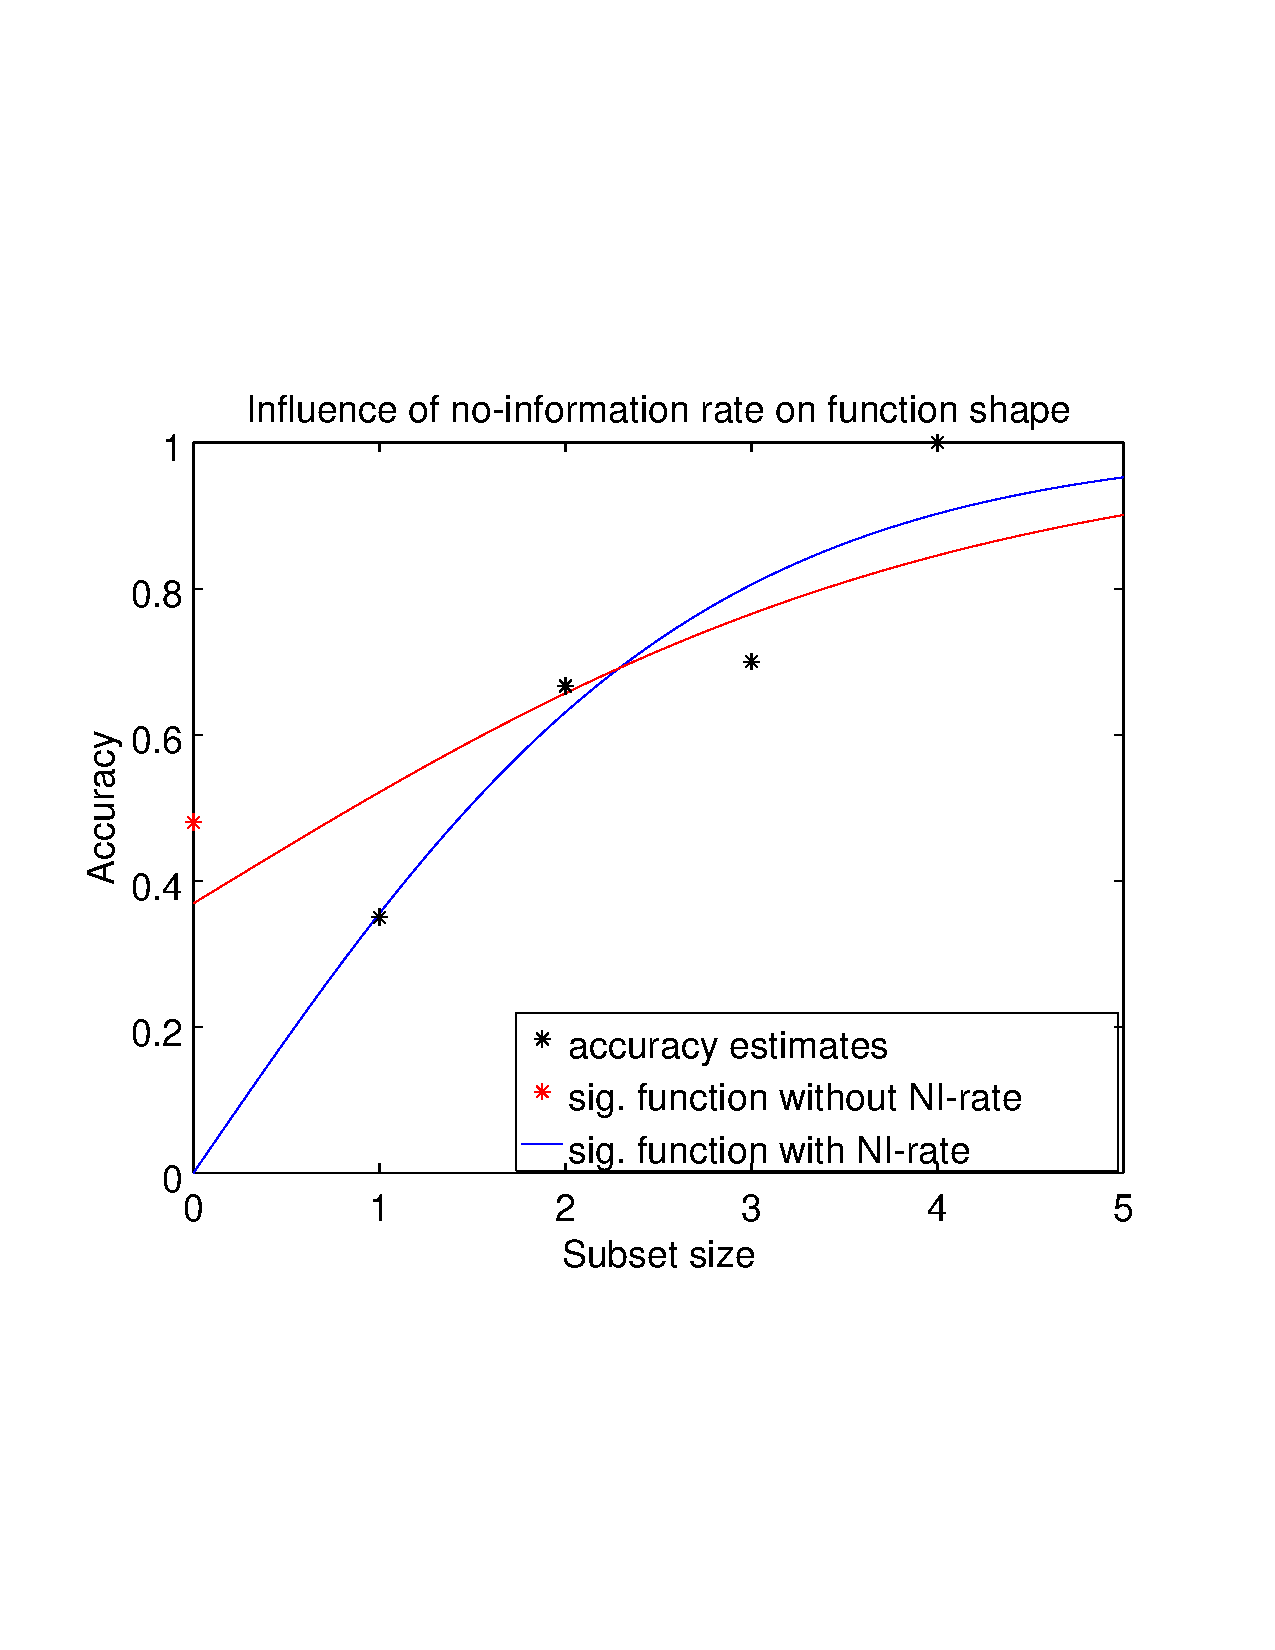
\includegraphics[trim = 1cm 7cm 1cm 6cm, clip = true, width = 0.48\textwidth]{fitNIRate}
	\caption{Difference of function shape for the sigmoid model when using weighting or the no-information rate}
	\label{fig:weigthingExample}
\end{figure}

Another potential improvement for the fitting process is the addition of data. Of course the number of subsets is fixed without purchasing more labels. But information not covered by leave-p-out may prove useful: showcased in \cite{EfronEtAl1997}, .632+ bootstrapping uses the \textit{no-information rate} to identify special overfit cases with data independent of its predictors. It is a heuristic used to approximate the error a classifier without any training would make when being tested on the dataset, the formula can be found in \ref{eq:niRate}. And while performance estimates for each subset size $|S^j_i| \in \{1, ..., k-1\}$ are available, the estimates do not yet include an estimate for $j = 0$, since most classifiers require at least one training instance to work. The no-information rate may be used as the 0th fitting point and usually slightly lifts the beginning of the function curve, as seen in \ref{fig:weigthingExample}, filling that gap and help primarily in scenarios with small $k$. For larger training sets, its influence should decrease as more regular estimates are available.